\chapter{Simulation}
In this chapter, results from ab-initio simulations are presented independent of experimental data. It turns out that a careful investigation of various phases of LSCO+O presents us with valuable clues regarding the average and local structure. The general strategy is to investigate the structure and dynamics within the DFT framework and use the results to discuss how and why DFT fails to describe the strongly correlated nature of cuprates.

One example of such comparison is shown in Chapter \ref{ch:anomaly}, where we can detect potentially interesting physics by following how experiments diverge from simulation. In this chapter we do a full suite of simulations including various dopants and electronic ground states in order to have a starting point for experimental studies.

\section{Crystal Structure}
The structural phases of lanthanum based cuprates fall into a moderate number of space groups as listed in Table \ref{tab:crystalstructures}. All of the structural phases can be described with reference to Figure \ref{fig:lscocrystal} where we define $Q_1$ as a rotation around the $[010]_o$ and $Q_2$ as a rotation around the $[100]_o$ axis. In our simulations we have chosen to focus mainly on the HTT, LTO and LTT phases, since they are the most common and give a good compromise when investigating the role of tilts $Q_1$, $Q_2$ and orthorhombic strain $\eta$.

\begin{table}
	\centering
	\begin{tabular}{@{}llll@{}}
		\toprule
		Space Group (\#) & Name (shorthand)                         & Tilts                                    & $\eta$   \\ \midrule
		I4/mmm (139)     & High-Temperature Tetragonal (HTT)        & $Q_1=Q_2=0$                              & $=0$     \\
		Fmmm (69)        &                                          & $Q_1=Q_2=0$                              & $\neq 0$ \\
		Bmab (64)        & Low-Temperature Orthorhombic (LTO)       & $Q_2 \neq 0$, $Q_1 = 0$                  & $\neq 0$ \\
		P4$_2$/ncm (138) & Low-Temperature Tetragonal (LTT)         & $Q_1=Q_2 \neq 0$                         & $=0$     \\
		Pccn (56)        & Low-Temperature-Less-Orthorhombic (LTLO) & $Q_1 \neq Q_2 \neq 0$ & $\neq 0$ \\ \bottomrule
	\end{tabular}
	\caption[Crystal structures LSCO]{Crystal structures found in various lanthanum-based cuprates. All structural phases can be parametrized with respect to LTLO, where $Q_1$ and $Q_2$ represent octahedral tilts as described in the text and $\eta=\frac{b-a}{b+a}$ is the orthorhombic strain.}
	\label{tab:crystalstructures}
\end{table}

\begin{figure}
	\centering
	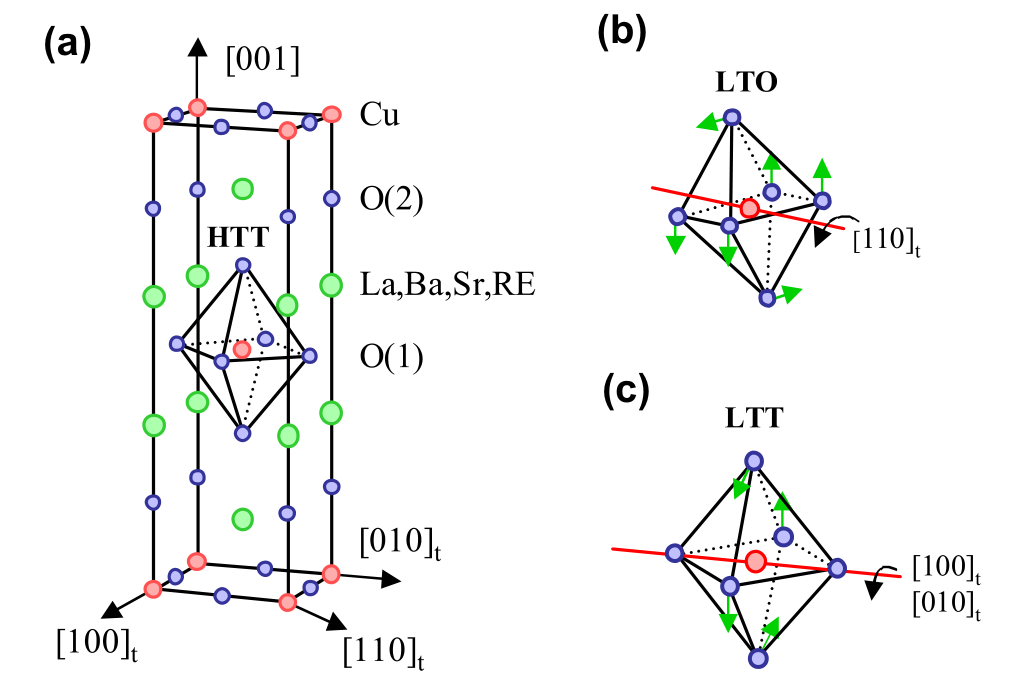
\includegraphics[width=0.8\textwidth]{fig/simulation/crystal_hucker.png}
	\caption[LSCO crystal]{Crystal structure of lanthanum based cuprates. From \cite{Hucker2012}. \todo[inline]{redo figure in orthorhombic coordinates with Q1 and Q2 as tilts}}
	\label{fig:lscocrystal}
\end{figure}

\subsection{Octahedral tilts}
In order to quantify the octahedral tilts, we use the coordinate system sketched in Figure \ref{fig:tilt}. All possible tilts can be described with reference to the LTLO (Pccn) phase. The octahedra are described with two in-plane oxygens (O$_1$, O$_2$) and one apical oxygen $O_3$. Due to symmetry constrains, a rotation of this octahedron will cause a displacements in the $c$-direction of the in-plane oxygen and in the $a$- and $b$-directions of the apical oxygen. Following \cite{Axe1989}, we define $Q_1$ as a rotation around the (010) axis and $Q_2$ as a rotation around the (100) axis in orthorhombic notation. In more intuitive terms, $Q_1$ `tilts' the octahedron along $x$, while $Q_2$ `tilts' along $y$.

\begin{figure}
	\centering
	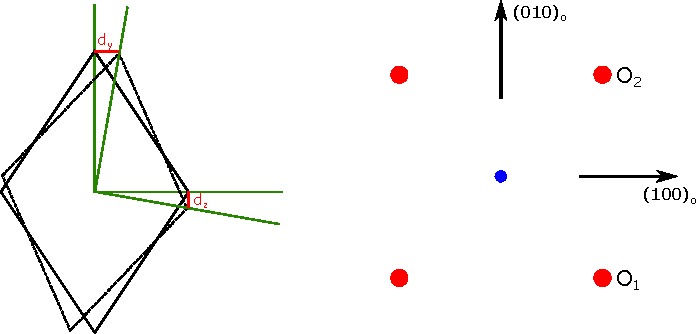
\includegraphics[width=0.8\textwidth]{fig/simulation/tilt.pdf}
	\caption[Geometry of octahedral tilts]{Left: Geometry of octahedral tilts in the with the $c$-axis vertical. Right: Illustration of the two inequivalent in-plane oxygens. The $Q_1$ irreducible representation represents a rotation around the (010) axis while $Q_2$ is a rotation around the (100) axis.\todo[inline]{could use an update}}
	\label{fig:tilt}
\end{figure}

By inspection of Figure \ref{fig:tilt}, a $Q_1$ rotation will displace O$_3$ in the $x$-direction and O$_1$, O$_2$ in the negative $z$-direction. A $Q_2$ rotation will displace O$_3$ in the $y$-direction, O$_1$ in the positive $z$-direction and O$_2$ in the negative $z$-direction. If we want to express $Q_1$ and $Q_2$ as angles, the displacements become:


\begin{align*}
d_x(\text{O}_3) &= | \text{O}_\text{ap} | \sin (Q_1) \frac{c}{a} \\
d_y(\text{O}_3) &= | \text{O}_\text{ap} | \sin (Q_2) \frac{c}{b} \\
d_z(\text{O}_1) &= \frac{1}{4c} \left[ - a \sin (Q_1) + b \sin (Q_2) \right] \\
d_z(\text{O}_2) &= \frac{1}{4c} \left[ - a \sin (Q_1) - b \sin (Q_2) \right] \, ,
\end{align*}

\noindent where $| \text{O}_\text{ap} |$ is the apical oxygen distance, or the $z$-component of O$_3$. Since these equations uniquely define displacements in terms of tilt angles, we can also find tilt angles from structural displacements from either the apical oxygen:

\begin{align*}
Q_1 &= \sin^{-1} \left( \frac{d_x(\text{O}_3)}{| \text{O}_\text{ap} |} \times \frac{a}{c} \right) \\
Q_2 &= \sin^{-1} \left( \frac{d_y(\text{O}_3)}{| \text{O}_\text{ap} |} \times \frac{b}{c} \right) \, ,
\end{align*}

\noindent or the equatorial oxygen:

\begin{align*}
Q_1 &= \sin^{-1}  \left( - \frac{2c}{a} \times (d_z(\text{O}_1) + d_z(\text{O}_2)) \right) \\
Q_2 &= \sin^{-1}  \left( -\frac{4c}{b} \times d_z(\text{O}_2) - \frac{a}{b} \times \sin (Q_1) \right) \, .
\end{align*}

\noindent These equations can then be used to generate desired tilts and extract tilt angles from any given structure.

\subsection{Band Structures}
Band structures are described with respect to the reciprocal lattice. Due to the enlargement of the real-space crystal structure as we move through HTT $\rightarrow$ LTO $\rightarrow$ LTT, the Brillouin Zone (BZ) shrinks by the same amount. Similar to how it is useful to describe our real-space lattice with respect to the LTLO coordinate system, it is useful to describe reciprocal space with respect to a common coordinate system when comparing results. As we can see in Figure \ref{fig:allbz}, the BZ's of HTT, LTO and LTT have vastly different shapes, so it is difficult to superimpose results.

\begin{figure}
	\centering
	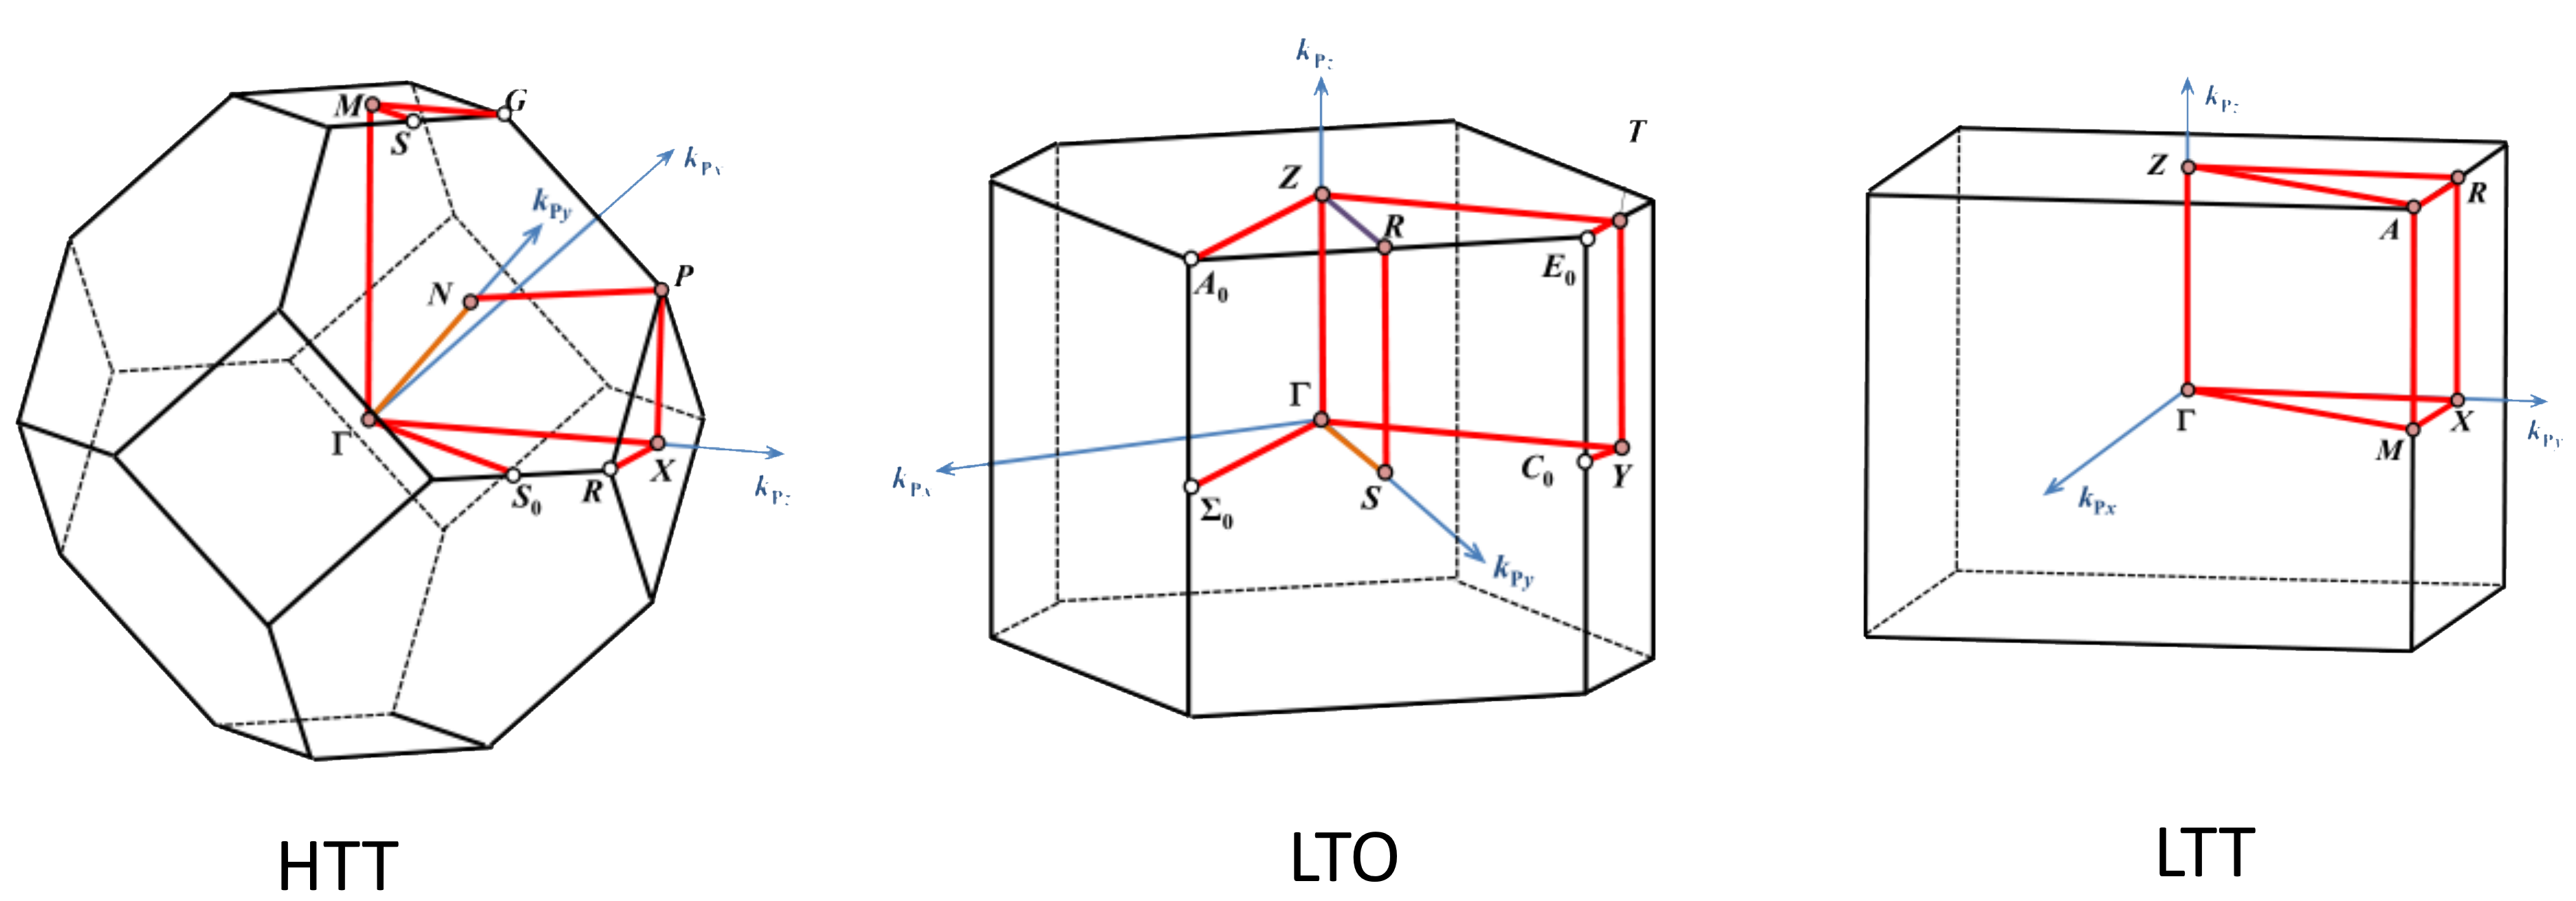
\includegraphics[width=0.8\textwidth]{fig/simulation/BZAll.png}
	\caption[HTT LTO LTT BZs]{BZ of the HTT, LTO and LTT phases. Modified from \todo[inline]{refer to hinuma paper}}
	\label{fig:allbz}
\end{figure}

For this reason, we chose a \emph{primitive} tetragonal BZ to describe the HTT phase and then construct the smaller LTO and LTT BZ's with respect to this construction. The idea is sketched in Figure \ref{fig:band_paths}. This construction also helps emphasize the 2-dimensional nature of the cuprates. In all following simulations, the band labels in Figure \ref{fig:band_paths} will be used, keeping in mind that the nature of high-symmetry points can change depending on the considered structural phase. One example is that the $M$ point, which is the zone boundary of HTT, becomes the zone center of LTO and would thus usually be denoted $\Gamma$.

\begin{figure}
    \centering
    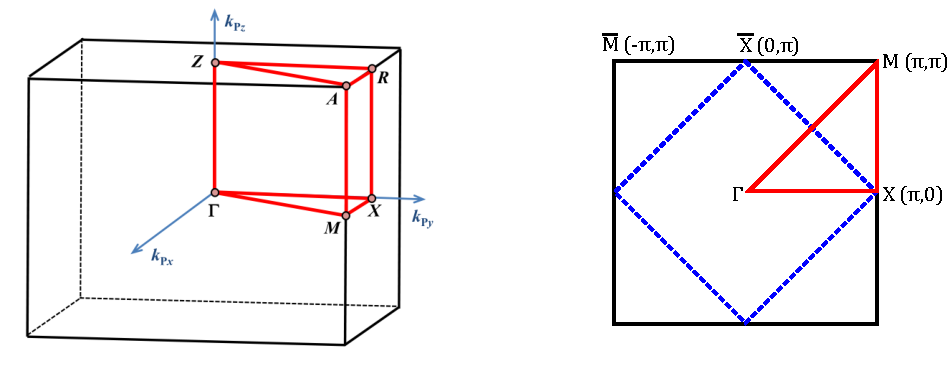
\includegraphics{fig/simulation/band_paths.pdf}
    \caption[Band paths]{\textbf{Left:} BZ of a primitive tetragonal cell with high-symmetry lines. \textbf{Right:} The in-plane BZ with the same labels and the usual $\Gamma$-$X$-$M$-$\Gamma$ path. If the large BZ is the crystallographic HTT phase, then the broken blue lines represent the LTO/LTT/LTLO BZ and we can consider the $\Gamma$-$X$-$\frac{M}{2}$-$\Gamma$ path, since $M$ becomes $\Gamma$ for this (smaller) BZ. In literature the labels are often confused, while $(\pi,\pi)$ and $(\pi,0)$ are universally agreed upon. In any band structure diagrams presented here, the labels in this figure is used.} 
    \label{fig:band_paths}
\end{figure}

While this construction is useful for our intuitive understanding of the different phases, most software expects $k$-vectors with respect to the primitive unit cell. For this reason, we need the transformation matrices from our constructed LTT coordinate system to the primitive HTT and LTO unit cells. This conversion can be done with the following matrices.

\[
\text{PA(HTT)} =  
\begin{pmatrix}
0 & 0 & \frac{1}{2} \\
\frac{1}{2} & \bar{\frac{1}{2}} & 0 \\
\frac{1}{2} & \frac{1}{2} & \bar{\frac{1}{2}}
\end{pmatrix}
\qquad
\text{PA(LTO)} =  
\begin{pmatrix}
\frac{1}{2} & \frac{1}{2} & 0 \\
0 & 0 & 1 \\
\frac{1}{2} & \bar{\frac{1}{2}} & 0
\end{pmatrix}
\]

\noindent these matrices can be used to generate $k$-points starting from the more `intuitive' notation outlined in Figure \ref{fig:band_paths}. For example, the $X$-point ($(\frac{1}{2} \frac{1}{2} 0)$ with respect to LTT) in the HTT phase becomes $(\frac{1}{2} \frac{1}{2} 0) \cdot \text{PA(HTT)} = (\frac{1}{4} \bar{\frac{1}{4}} \frac{1}{4})$.\todo{Double-check this. It works for the band structures, but still not sure why. Relation to real-space transformation matrices?}

\section{VASP Simulation details}
All DFT simulations\todo{refer to method} are performed using the Vienna Ab-Initio Simulation Package (VASP)\todo{several refs}. While ab-initio loosely translates to `from the beginning', There are several choices to be made with regards to computational parameters. First, we need to define the pseudo-potentials that describes the valence electrons of each atomic species in our system. For LCO, the relevant pseudo-potentials are listed in Table \ref{tab:vasp_pseudo} along with their electronic configuration. For both La and O we used the recommended potentials, while for Cu we used a more accurate version where 3p electrons are included (\verb|_pv| is short for `p in valence').


\begin{table}[b]
\centering
\begin{tabular}{@{}lll@{}}
\toprule
 & Core (\# electrons) & Valence (\# electrons)                        \\ \midrule
\texttt{La}                 & Kr4d$^{10}$ (46)                & 5s$^1$6s$^2$5p$^6$5d$^1$ (11) \\
\texttt{Sr\_sv} & (28) & 4s$^2$4p$^6$5s$^2$ (10) \\
\texttt{Cu\_pv}                 & 1s$^2$2s$^2$2p$^6$3s$^2$ (12) & 3p$^6$3d$^{10}$4s$^1$ (17)      \\
\texttt{O}                  & 1s$^2$ (2)                    & 2s$^2$2p$^4$ (6)              \\ \bottomrule
\end{tabular}
\caption[VASP Pseudopotentials]{Psedopotenial electronic configuration used in VASP calculations.\todo[inline]{Check Sr potential}}
\label{tab:vasp_pseudo}
\end{table}

A VASP simulations requires 4 distinct files to run. The \texttt{POSCAR} file defines the lattice and fractional coordinates. The \texttt{POTCAR} files contains the pseudo-potentials. The \texttt{KPOINTS} file determines the $k$-point sampling mesh. Finally \texttt{INCAR} gives the computational parameters. A minimal \texttt{INCAR} file for VASP is shown in Figure \ref{fig:incar}. Depending on the type of simulation, parameters may be added or changed. It is not always straightforward to chose an optimal set of parameters since it depends heavily on the type of problem, system size and available computational resources.

\begin{figure}
    \centering
    \begin{lstlisting}[basicstyle=\footnotesize\ttfamily, frame=single]
    ENCUT = 520 # 1.3x suggested value from O POTCAR, 800 for phonons
    EDIFF = 1E-5 # 1E-8 for phonons
    ALGO = NORMAL
    PREC = Accurate
    ADDGRID = .FALSE.
    LREAL = Auto # Switch to .FALSE. for phonons
    
    GGA = PS # PBESol functional, PE switches to default PBE
    
    ISPIN = 2
    MAGMOM = 1 -1 1 -1 24*0 # AFM structure
    
    IBRION = -1 # Single point calculation
    NSW = 0     # Number of ionic steps
    
    ISMEAR = 0
    SIGMA = 0.1
    
    LDAU= .TRUE. # Enable LDA+U with U=8eV and J=0.8eV
    LDAUTYPE = 4 # No exchange splitting
    LDAUL = 2 -1 -1 # only on Cu d states
    LDAUU = 8 0 0 
    LDAUJ = 0.8 0 0
    \end{lstlisting}
    \caption[VASP: Typical INCAR]{Typical INCAR for VASP simulations.}
    \label{fig:incar}
\end{figure}

\section{Benchmarking}
When performing DFT calculations in VASP there are a few parameters that have significant impact on the precision of the calculation. Increasing the precision also results in significantly longer computation time, so it is important to find a compromise. 

Figure \ref{fig:sim_bench_afm} shows a benchmark of AFM LCO with respect to the $k$-point mesh and smearing width $\sigma$. Since there are no states at the Fermi level, the smearing width converges rather quickly, and we can safely use a value of $\sigma = \SI{0.1}{\eV}$. The $k$-point density also converges rather quickly, and we achieve a precision of \SI{0.1}{\milli\eV} using a fairly coarse MP-grid of $8\times 8 \times 4$. In AFM LCO we also checked the effect on electronic structure due to the on-site repulsion $U$. The result is shown in Table \ref{tab:ldau}

\begin{figure}
    \centering
    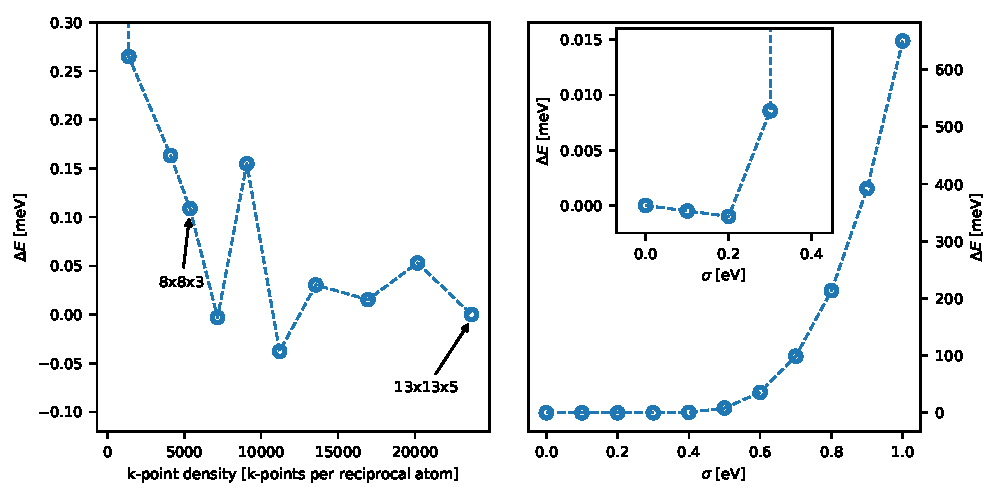
\includegraphics{fig/simulation/convergence_afm.pdf}
    \caption[Simulation Benchmarks: GGA+U]{Simulation Benchmarks: GGA+U with $U=\SI{8}{\eV}$ and $J=\SI{0.8}{\eV}$. \textbf{Left:} Energy as a function of k-point density with $\sigma=\SI{0.1}{\eV}$. $\Delta E$ is total energy (with entropy) with respect to the $13 \times 13 \times 5$ mesh. \textbf{Right:} $\Delta E$ as a function of smearing $\sigma$, where $\sigma=0$ corresponds to the tetrahedron method (\texttt{ISMEAR=-5}).}
    \label{fig:sim_bench_afm}
\end{figure}

\begin{table}[b]
	\centering
	\begin{tabular}{@{}llll@{}}
		\toprule
		U [eV] & J [eV] & Moment [$\mu_\text{B}$] & Optical gap [eV] \\ \midrule
		4.0    & 0.4    & 0.330       & 0.348    \\
		6.0    & 0.6    & 0.481       & 1.016    \\
		8.0    & 0.8    & 0.588       & 1.686    \\
		10.0   & 1.0    & 0.676       & 1.877    \\
		12.0   & 1.2    & 0.755       & 2.042    \\ \bottomrule
	\end{tabular}
	\caption[LDA+U Benchmarking]{LDA+U Benchmarking}
	\label{tab:ldau}
\end{table}

Due to partial occupancies, metallic systems are generally more sensitive to $k$-point density and smearing width/method. For this reason, we performed a more comprehensive set of benchmarks as shown in Figure \ref{fig:sim_bench_para}. While the numerical fluctuations are still within a few meV, the precision on total energy is decreased by a few orders of magnitude.

\begin{figure}
    \centering
    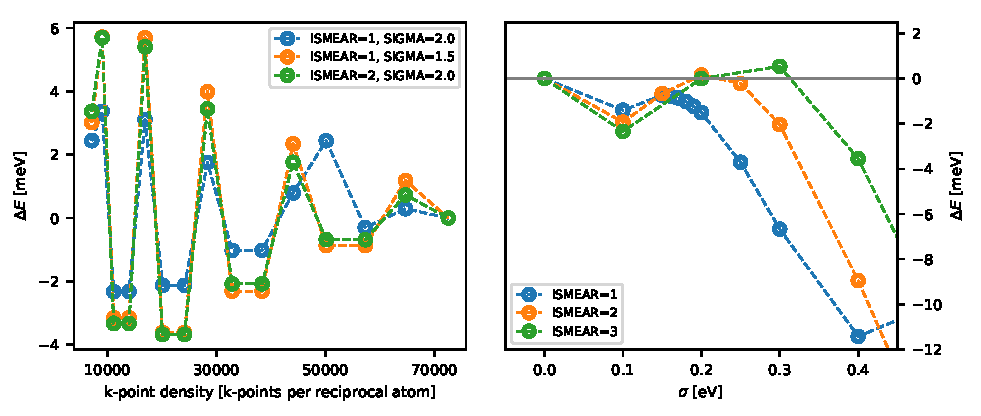
\includegraphics{fig/simulation/convergence_metal.pdf}
    \caption[Simulation Benchmarks: Paramagnet/Metal]{Simulation Benchmarks: Paramagnet/Metal. Note the significant variation in energy compared to the insulating case, even with much higher k-point density. \textbf{Left:} Energy as a function of k-point density for three combinations values of $\sigma$ and smearing type. $\Delta E$ is total energy (with entropy) with respect to the $18 \times 18 \times 8$ mesh. \textbf{Right:} $\Delta E$ as a function of $\sigma$ with the Methfessel-Paxton method (orders 1, 2, 3) while using a $16 \times 16 \times 8$ k-point mesh (57344 k-points per reciprocal atom). $\sigma=0$ corresponds to the tetrahedron method (\texttt{ISMEAR=-5}). Below $\sigma = \SI{0.4}{\eV}$ the entropy term is \SI{0.5}{\milli\eV} per atom or lower, so forces should be well-behaved.}
    \label{fig:sim_bench_para}
\end{figure}

%\begin{table}[b]
%	\centering
%	\begin{tabular}{@{}lllll@{}}
%		\toprule
%		& HTT & HTT (metal)  & LTO    & LTT    \\ \midrule
%		a [\AA]         & 5.32 & 5.31 & 5.34   & 5.37   \\
%		c [\AA]         & 12.99 & 13.05 & 13.01  & 12.93  \\
%		O3(z)      & 0.184 & 0.185 & 0.185  & 0.184  \\
%		La(x)      & 0     & 0 & 0      & -0.009 \\
%		La(y)      & 0     & 0 & -0.012 & -0.009 \\
%		La(z)      & 0.362 & 0.362 & 0.361  & 0.361  \\
%		$\eta$ ($\times 100$) & 0  & 0 &  1.465  & 0      \\
%		Q1 (degrees)        & 0 & 0 &  0      & 4.6125 \\
%		Q2 (degrees)        & 0 & 0 &  5.786  & 4.6125 \\ 
%		degrees of freedom & 2 & 2 & 5 & 5 \\ \bottomrule
%	\end{tabular}
%	\caption[HTT, LTO, LTT: Structural parameters]{HTT, LTO, LTT: Structural parameters, defined with a minimal set of parameters based on results from simulations. Q1/Q2 are taken as the average angle from equatorial and apical tilt. The fractional positions of O1, O2 and O3 are completely described using Q1, Q2 and O3(z), Cu is allways at (0,0,0) and $\eta = \frac{b-a}{b+a}$ uniquely defines any difference between $a$ and $b$. In the generation of structures, the Pccn (LTLO) space group is used. Degrees of freedom refers to the atomic positions only. The description of our system in terms of Q1/Q2 thus removes one degree of freedom by coupling the apical and equatorial oxygen.}
%	\label{tab:struct_par}
%\end{table}

\section{Electronic Structure}
While we are generally interested in lattice dynamics, a DFT calculation is leveraging the electronic structure in any simulation. It is thus worthwhile to check if the electronic structure, at least approximately, represents reality. In the cuprates, it is well known that DFT is unable to explain the peculiarities in the superconducting phase. However, we can get fairly close in the limit of zero doping (AFM Mott Insulator) and overdoping (fermi liquid). Figure \ref{fig:edos_htt} compares the electronic density of states of the Mott Insulator and fermi liquid for two different functionals. We clearly see how the DFT+U opens a gap by pushing states below the Fermi level.

\begin{figure}
    \centering
    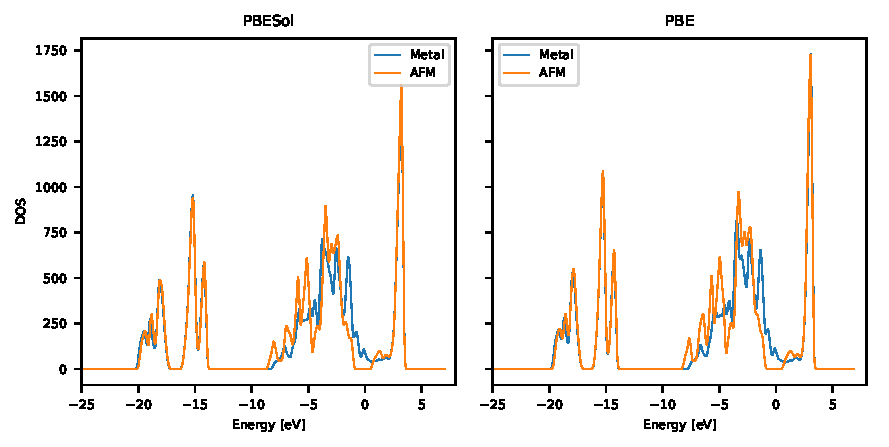
\includegraphics{fig/simulation/htt_dos.pdf}
    \caption[Electronic DOS: Metal and AFM]{Electronic density of states for HTT phase with two different functionals in a metallic (paramagnetic) and AFM (GGA+U) states. The two functionals appear to describe the system identically. The AFM state is shifted by \SI{-1}{\eV} for comparative purposes (which is why the Fermi level is in the middle of the gap).}
    \label{fig:edos_htt}
\end{figure}

To further illustrate this point, Figure \ref{fig:bs_afm2} and \ref{fig:bs_metal} shows the band structure coloured by atomic projections in the AFM and metallic state, respectively. We now notice that DFT+U is pushing the Cu states down, as expected from the on-site respulsion.

\begin{figure}
    \centering
    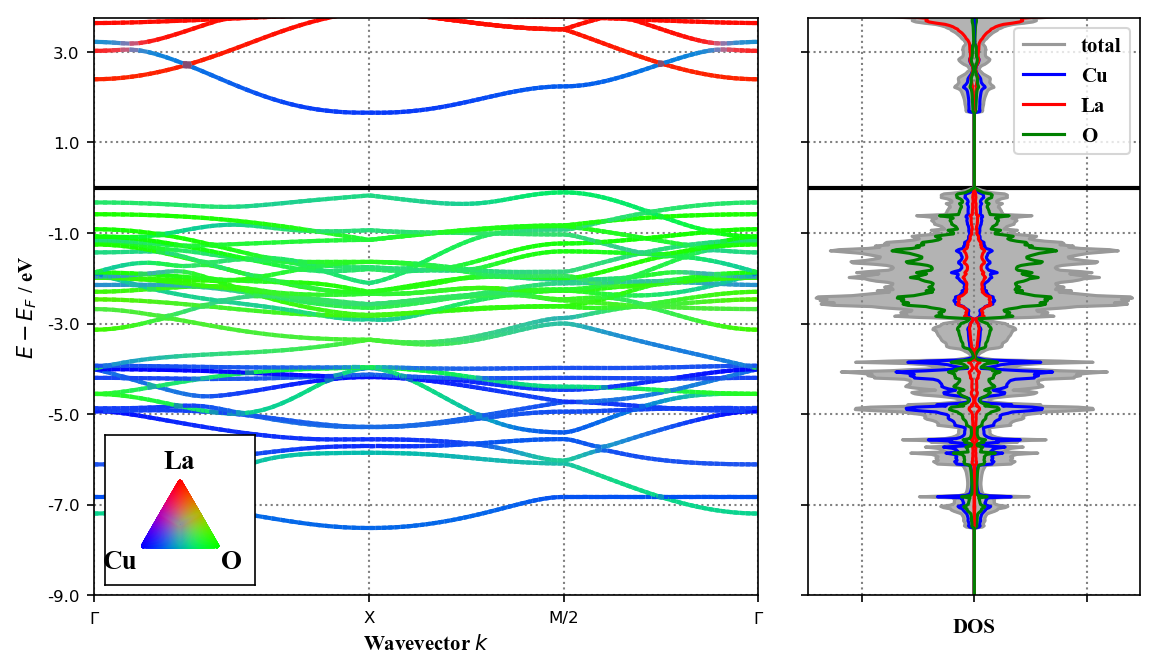
\includegraphics[width=\textwidth]{fig/simulation/bs_afm2.png}
    \caption[GGA+U: AFM Electronic Band Structure]{GGA+U: AFM Electronic Band Structure of the Bmab LTO structure along the $\Gamma$-$X$-$\frac{M}{2}$-$\Gamma$ path (LTO high symmetry lines). The upper and lower Hubbard bands are clearly visible and are separated by \SI{8}{\eV} as expected.}
    \label{fig:bs_afm2}
\end{figure}

%\begin{figure}
%    \centering
%    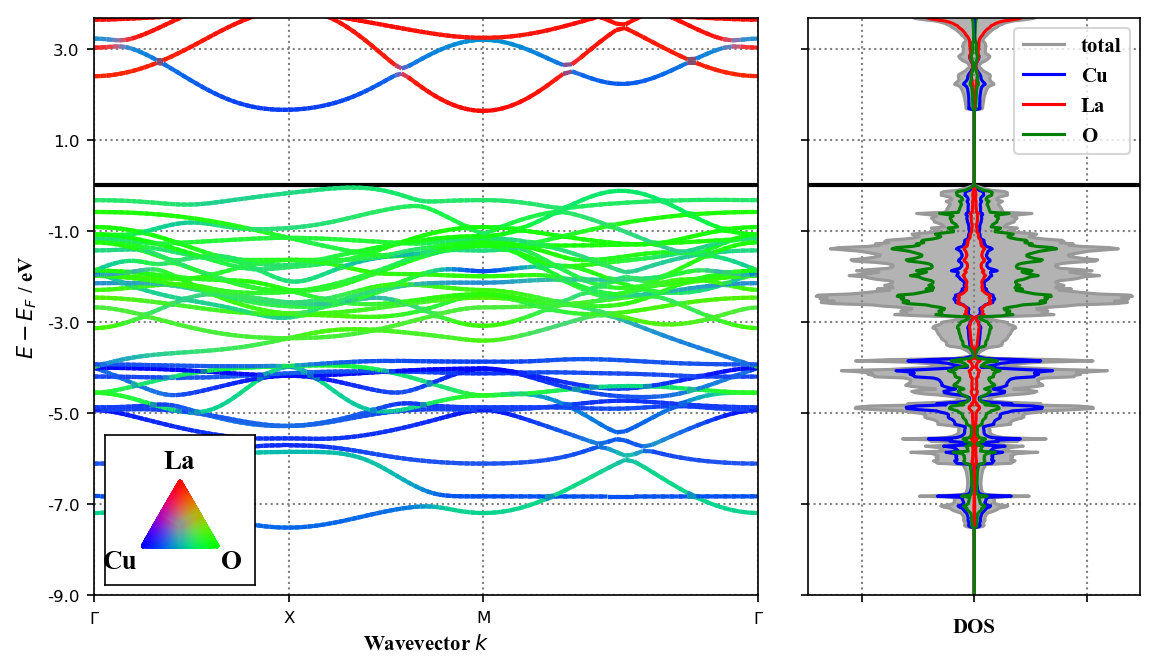
\includegraphics[width=\textwidth]{fig/simulation/bs_afm1.png}
%    \caption[GGA+U: AFM Electronic Band Structure]{GGA+U: AFM Electronic Band Structure of the Bmab LTO structure along the $\Gamma$-$X$-$M$-$\Gamma$ path (HTT high symmetry lines). The upper and lower Hubbard bands are clearly visible and are separated by \SI{8}{\eV} as expected.}
%    \label{fig:bs_afm1}
%\end{figure}

\begin{figure}
    \centering
    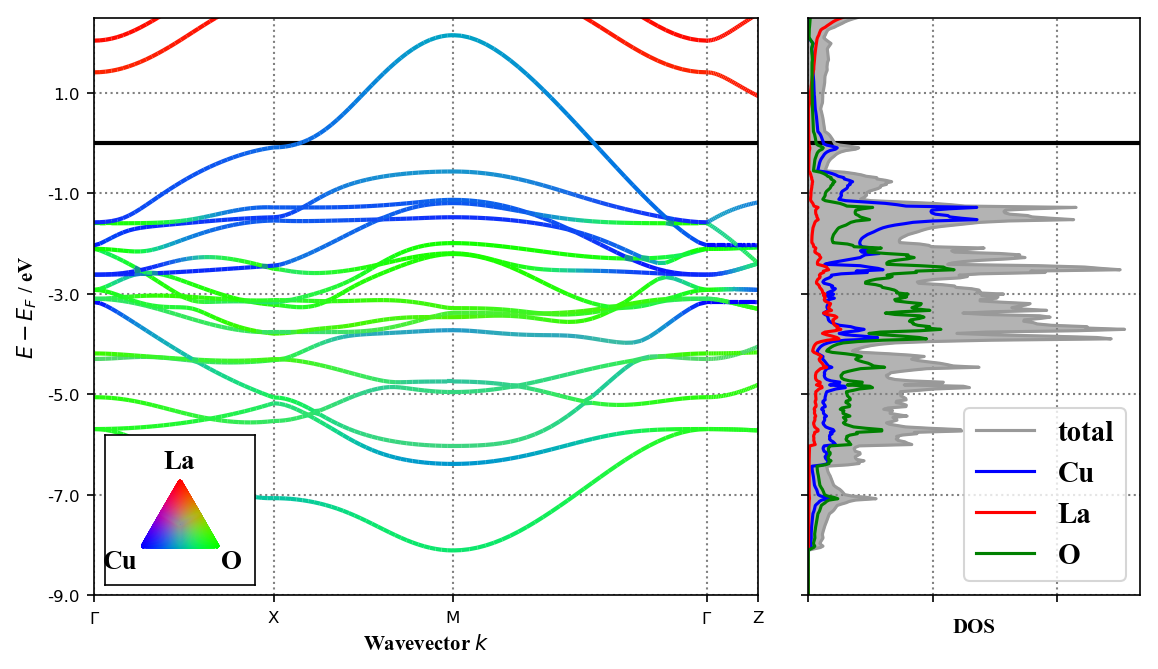
\includegraphics[width=\textwidth]{fig/simulation/bs_metal.png}
    \caption[GGA: Metallic Electronic Band Structure]{Metallic Electronic Band Structure of the I4/mmm HTT structure. Path is through the high-symmetry points as defined in Figure \ref{fig:band_paths} with respect to the conventional unit cell. The $\Gamma$-$Z$ path is shown to illustrate the 2-dimensional nature of the electronic structure (The dispersion is relatively flat).}
    \label{fig:bs_metal}
\end{figure}

\section{Geometry optimization}

\begin{figure}
    \centering
    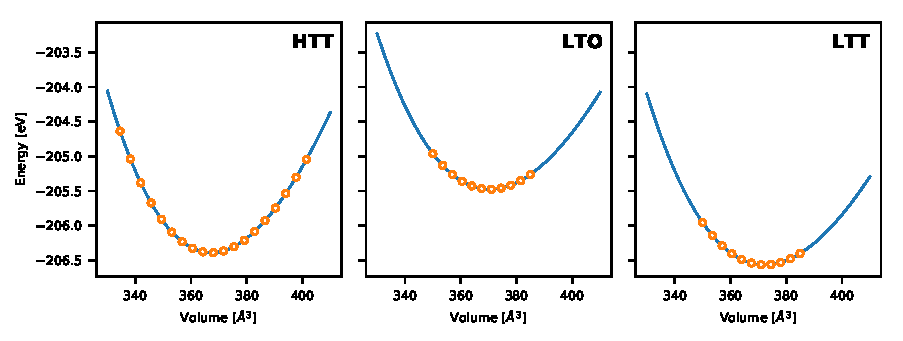
\includegraphics[width=\textwidth]{fig/simulation/eos_all.pdf}
    \caption[AFM: Equation-of-state fits]{Equation-of-state fits (AFM). Optimal volume of simulated structures are found by performing optimization of fractional coordinates and cell shape at a series of fixed volumes. The resulting Energy/Volume curve is then fit to a Vinet exponential equation of state \cite{Vinet1987}. This is done for the HTT, LTO and LTT phases with the PBESol functional.}
    \label{fig:eos_all}
\end{figure}

\begin{figure}
    \centering
    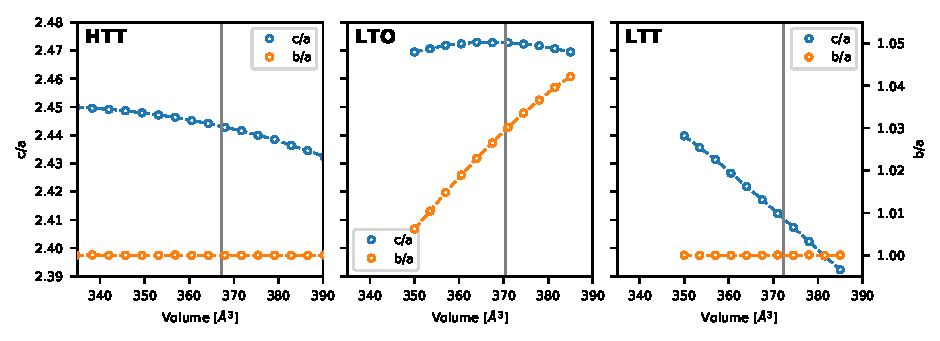
\includegraphics[width=\textwidth]{fig/simulation/ratio_all.pdf}
    \caption[AFM: Cell ratios during EOS fits]{Cell Ratios (AFM). During the equation-of-states fits from Figure \ref{fig:eos_all}, the cell shape is modified, changing the $b/a$ ratio (orthorhombicity) and $c/a$ ratio (larger values correspond to a cell that is elongated along $c$). Due to symmeetry $b/a = 1$ for the HTT and LTT phases. Vertical line is the optimal volume from the fit.}
    \label{fig:eos_ratios}
\end{figure}

\begin{figure}
    \centering
    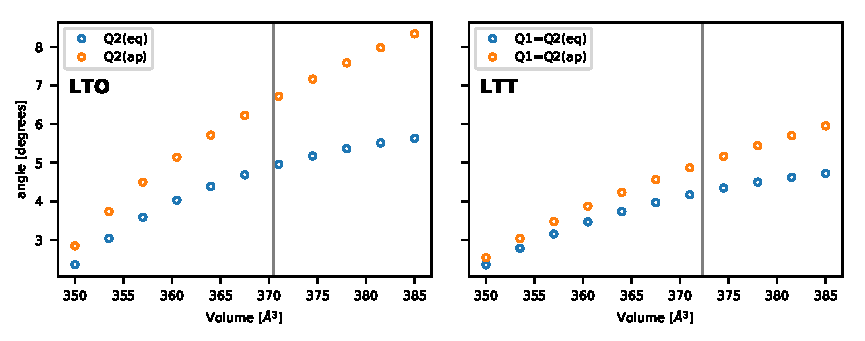
\includegraphics[width=\textwidth]{fig/simulation/angles_lto_ltt.pdf}
    \caption[AFM: LTO/LTT angles during EOS fits]{LTO/LTT Angles (AFM) During equation-of-state fits (Figure \ref{fig:eos_all}, we record the tilt angles for the LTO and LTT phase. Here, they are plotted as a function of Volume. Note that for LTO $Q_1=0$ and for LTT $Q_1=Q_2$. However, the rotation angle is measured differently from the equatorial (eq) and apical (ap) oxygen. The difference in values can be thought of as `non-rigidity' of the rotation.}
    \label{fig:my_label}
\end{figure}


\begin{figure}
    \centering
    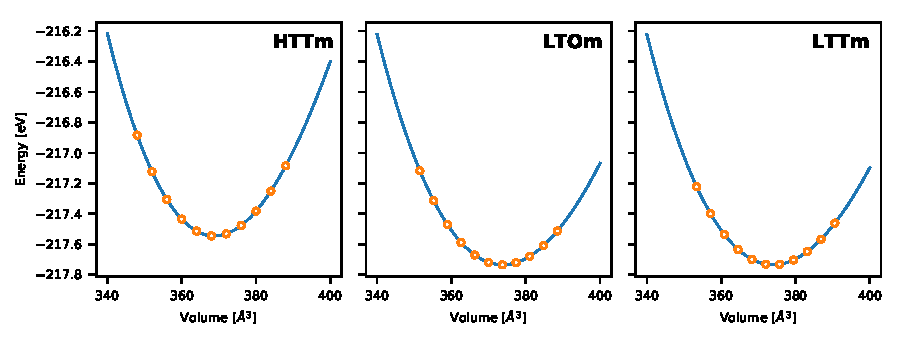
\includegraphics[width=\textwidth]{fig/simulation/eos_metal_all.pdf}
    \caption[Metal: Equation-of-state fits]{Equation-of-state fits (Metal). Optimal volume of simulated metallic structures are found by performing optimization of fractional coordinates and cell shape at a series of fixed volumes. The resulting Energy/Volume curve is then fit to a Vinet exponential equation of state \cite{Vinet1987}. This is done for the HTT, LTO and LTT phases with the PBESol functional.}
    \label{fig:eos_metal_all}
\end{figure}

\begin{figure}
    \centering
    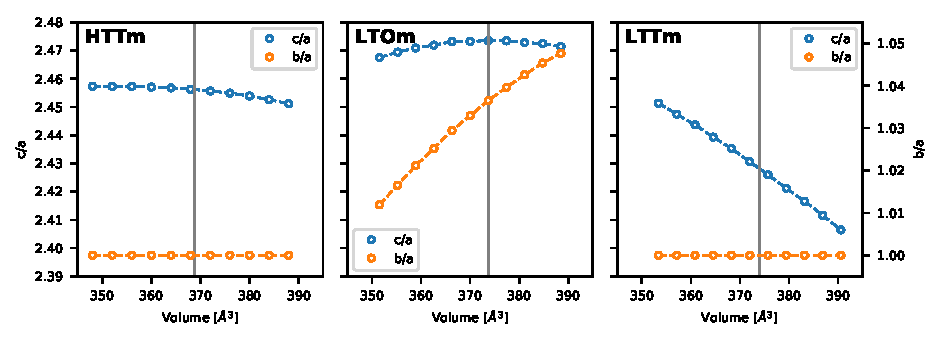
\includegraphics[width=\textwidth]{fig/simulation/ratio_metal_all.pdf}
    \caption[Metal: Cell ratios during EOS fits]{Cell ratios (Metal). During the equation-of-states fits from Figure \ref{fig:eos_metal_all}, the cell shape is modified, changing the $b/a$ ratio (orthorhombicity) and $c/a$ ratio (larger values correspond to a cell that is elongated along $c$). Due to symmeetry $b/a = 1$ for the HTT and LTT phases. Vertical line is the optimal volume from the fit.}
    \label{fig:eos_ratios}
\end{figure}

\begin{figure}
    \centering
    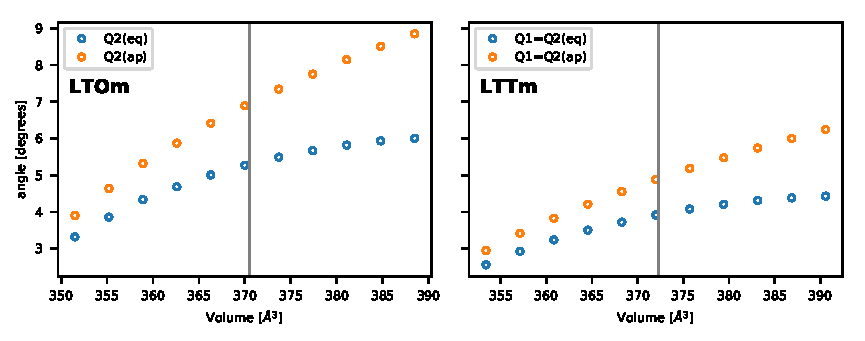
\includegraphics[width=\textwidth]{fig/simulation/angles_metal_lto_ltt.pdf}
    \caption[Metal: LTO/LTT angles during EOS fits]{LTO/LTT angles (Metal). During equation-of-state fits (Figure \ref{fig:eos_all}, we record the tilt angles for the LTO and LTT phase. Here, they are plotted as a function of Volume. Note that for LTO $Q_1=0$ and for LTT $Q_1=Q_2$. However, the rotation angle is measured differently from the equatorial (eq) and apical (ap) oxygen. The difference in values can be thought of as `non-rigidity' of the rotation.}
    \label{fig:my_label}
\end{figure}

\begin{table}[b]
    \centering
    \begin{tabular}{lllllllllll}
\toprule
structure &  phase & encut &      XC &       E0 &       V0 &    c/a &    $\eta$ &     $Q_1$ &     $Q_2$ \\
\midrule
      HTT &    afm &   520 &     PBE & -194.352 &  383.410 &  2.431 &  0.000 &  0.000 &  0.000 \\
      HTT &    afm &   800 &     PBE & -194.494 &  383.297 &  2.430 &  0.000 &  0.000 &  0.000 \\
      HTT &    afm &   800 &  PBESol & -206.390 &  367.310 &  2.443 &  0.000 &  0.000 &  0.000 \\
      LTO &    afm &   800 &  PBESol & -205.476 &  370.500 &  2.437 &  1.465 &  0.000 &  5.786 \\
      LTT &    afm &   800 &  PBESol & -206.565 &  372.282 &  2.410 &  0.000 &  4.612 &  4.612 \\
      HTT &  metal &   800 &  PBESol & -217.546 &  368.774 &  2.456 &  0.000 &  0.000 &  0.000 \\
      LTO &  metal &   800 &  PBESol & -217.735 &  373.793 &  2.430 &  1.795 &  0.000 &  6.421 \\
      LTT &  metal &   800 &  PBESol & -217.735 &  373.948 &  2.428 &  0.000 &  4.528 &  4.528 \\
\bottomrule
\end{tabular}

    \caption[Simulation Structure Results]{Resulting structure due to EOS fits to various structural phases and functionals. The two values given for $Q_1$/$Q_2$ are angles calculated from equatorial and apical oxygens, respectively. Interestingly, in terms of energy LTT $<$ HTT $<$ LTO, while the phonons are `more unstable' for HTT than LTO (See Figures \ref{fig:htt_ps}, \ref{fig:lto_ps}, \ref{fig:ltt_ps}). For the metallic cases, we note the optimal geometry is similar to the magnetic case. While the energy is lower, it is not meaningful to compare total energies between GGA+U and GGA.}
    \label{tab:sim_struct}
\end{table}

\begin{figure}
    \centering
    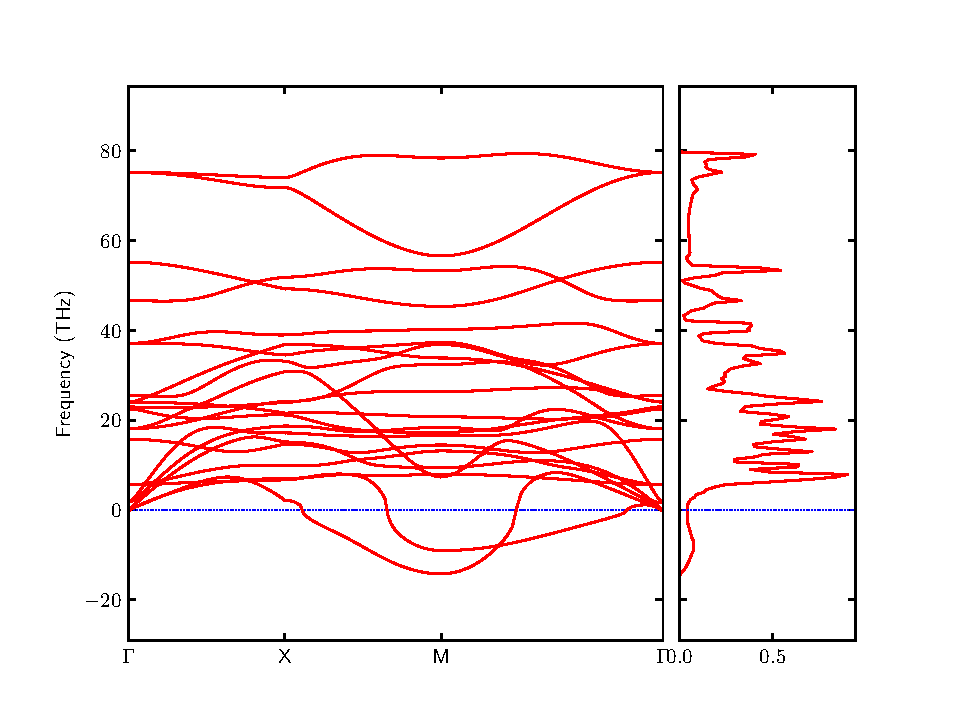
\includegraphics[width=\textwidth]{fig/simulation/band_dos_htt_pe.pdf}
    \caption[HTT Phonons (PBE)]{Phonons in HTT phase with PBE functional. Units are meV (the label is wrong). Note the problems with $\Gamma$ phonons.}
    \label{fig:htt_pe}
\end{figure}

\begin{figure}
    \centering
    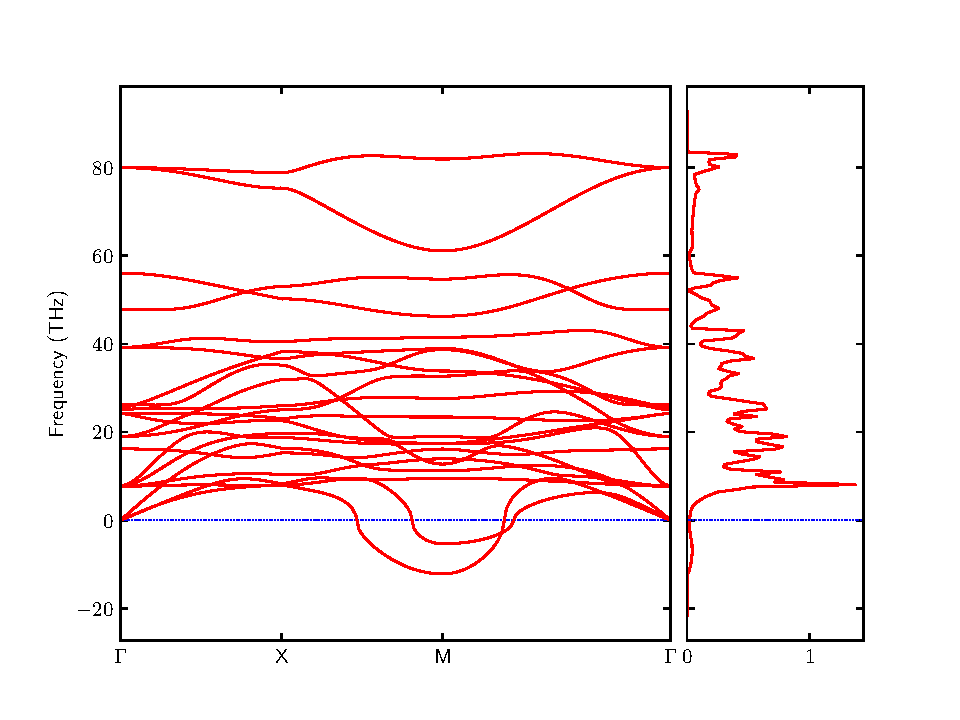
\includegraphics[width=\textwidth]{fig/simulation/band_dos_htt_ps.pdf}
    \caption[HTT Phonons (PBESol)]{Phonons in HTT phase with PBESol functional. Units are meV (the label is wrong). Note $\Gamma$ phonons are fixed.}
    \label{fig:htt_ps}
\end{figure}

\begin{figure}
    \centering
    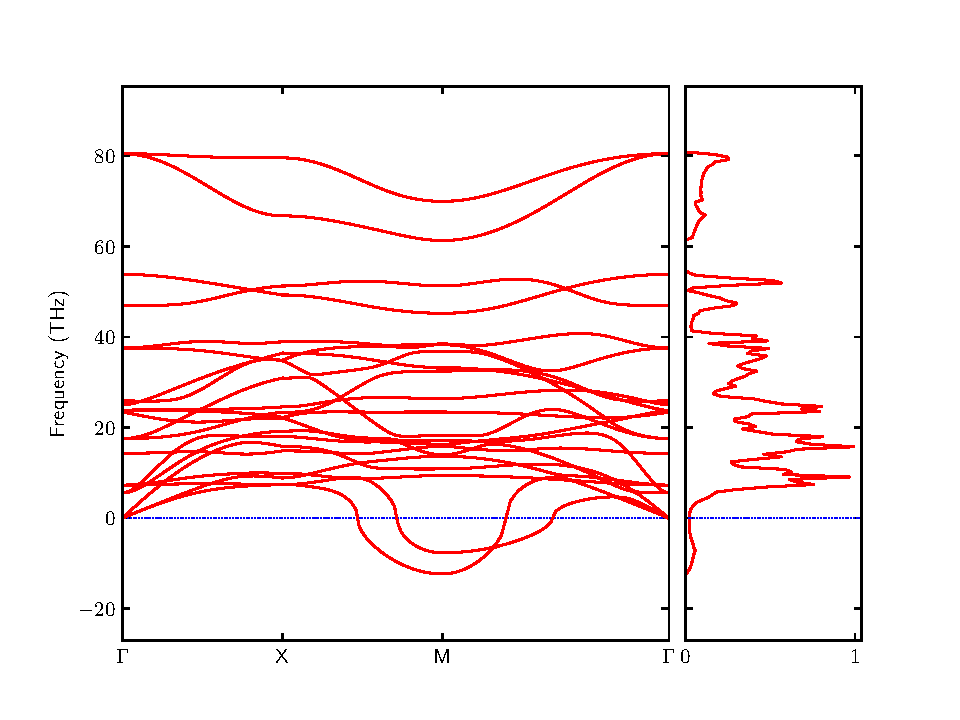
\includegraphics[width=\textwidth]{fig/simulation/band_dos_htt_metal.pdf}
    \caption[HTT Phonons (PBESol, Metal)]{Metallic Phonons in HTT phase with PBESol functional. Units are meV (the label is wrong). Note $\Gamma$ phonons are fixed.}
    \label{fig:htt_metal_ph}
\end{figure}

\begin{figure}
    \centering
    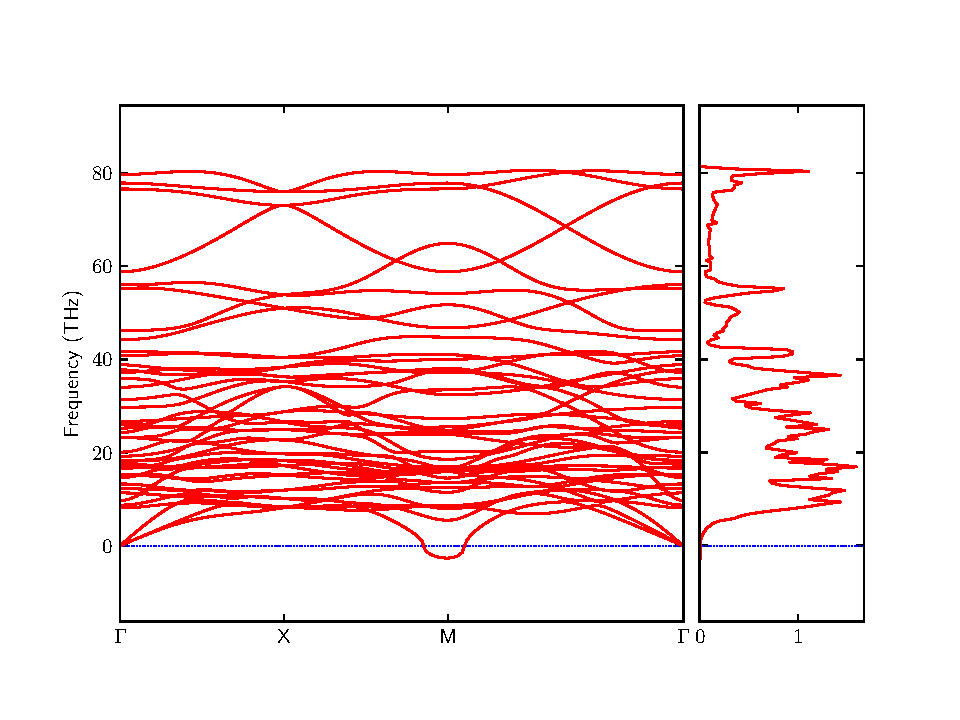
\includegraphics[width=\textwidth]{fig/simulation/band_dos_lto.pdf}
    \caption[LTO Phonons (PBESol)]{Phonons in LTO phase with PBESol functional. Units are meV (the label is wrong).}
    \label{fig:lto_ps}
\end{figure}

\begin{figure}
    \centering
    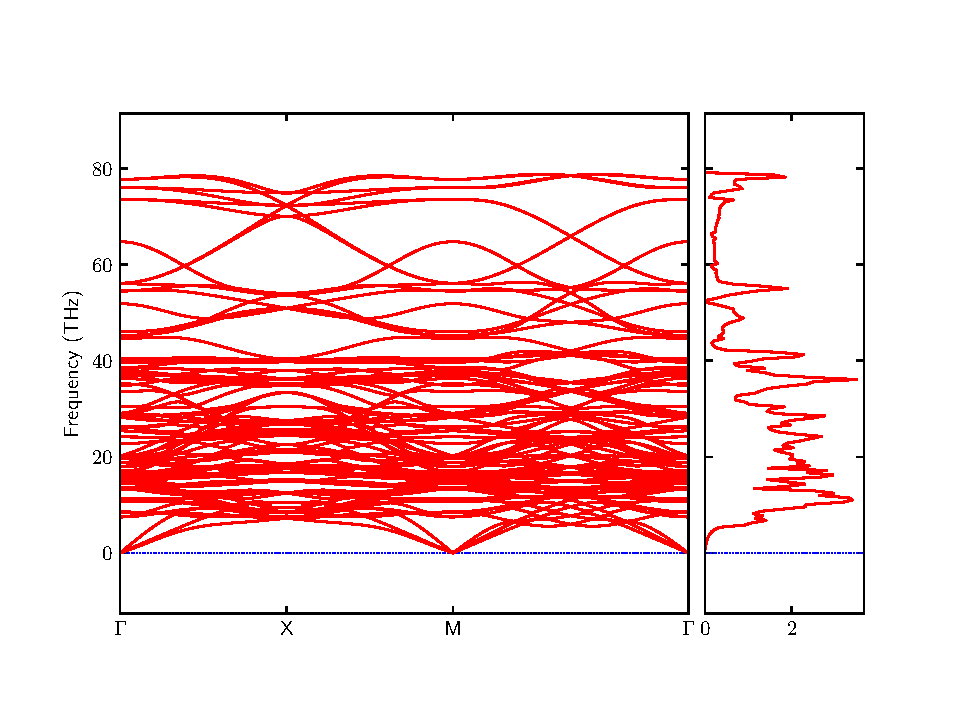
\includegraphics[width=\textwidth]{fig/simulation/band_dos_ltt.pdf}
    \caption[LTT Phonons (PBESol)]{Phonons in LTT phase with PBESol functional. Units are meV (the label is wrong).}
    \label{fig:ltt_ps}
\end{figure}

\begin{figure}
    \centering
    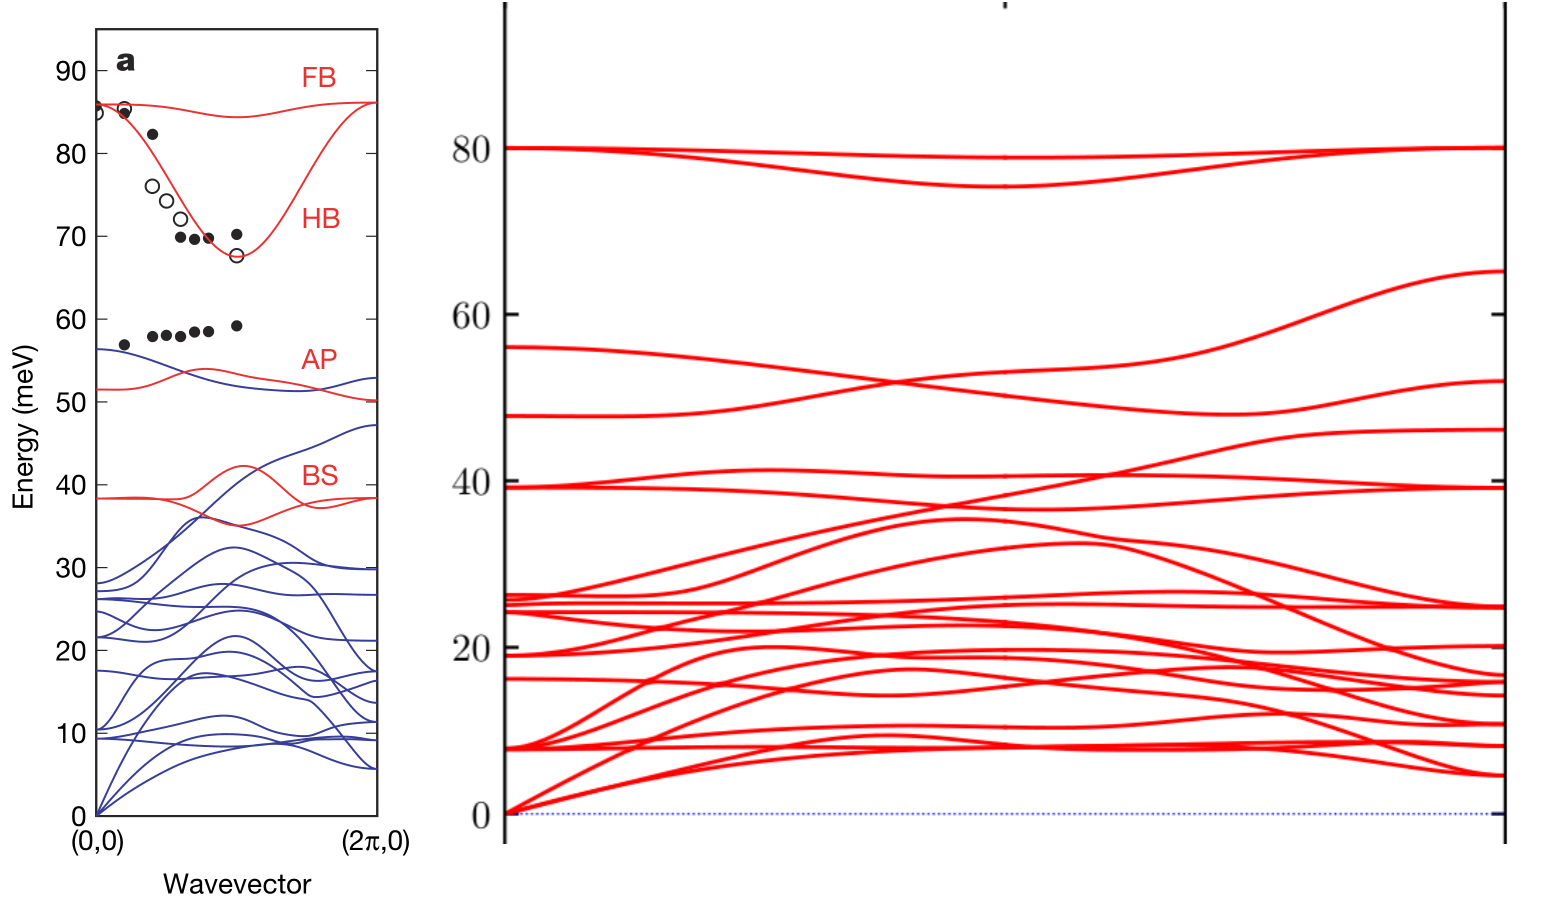
\includegraphics[width=\textwidth]{fig/simulation/giu_compare.png}
    \caption{Comparison of our AFM I4/mmm phonon dispersion with giustino et al. metallic phonons including e-ph coupling.}
    \label{fig:giu_compare}
\end{figure}



\begin{figure}
    \centering
    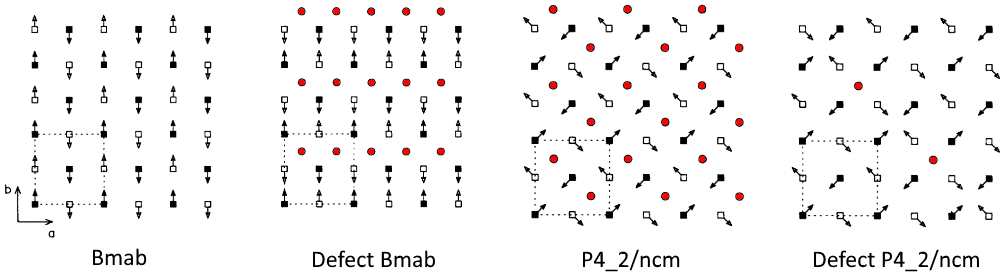
\includegraphics[width=\textwidth]{fig/simulation/oint.png}
    \caption[Illustration of interstitial positions]{Illustration of interstitial oxygen in-plane ($a$-$b$) location with respect to the apical oxygen displacements in the rock-salt layer. Open squares represent apical oxygens `hanging down' while closed squares represent apical oxygens `sticking up'. Interstitial oxygen are red circles. Adapted from \cite{Tranquada1995}.}
    \label{fig:oint_location}
\end{figure}

\begin{table}[b]
    \centering
    \begin{tabular}{@{}lllll@{}}
\toprule
Phase                   & Space Group & $\text{O}_\text{i}^x$ & $\text{O}_\text{i}^y$ & $\text{O}_\text{i}^z$ \\ \midrule
HTT                     & I4/mmm (139)      &         &         &         \\
HTT + O$_\text{i}$      & P-42m  (111)    & 0.125   & 0.125   & 0.25    \\
HTT + O$_\text{i}$      & Cmm2 (35)       & 0.125   & 0.125   & 0.24    \\
LTO                     & Bmab (64)       &         &         &         \\
LTO + O$_\text{i}$      & P2 (3)    & 0.125   & 0.125   & 0.25    \\
LTO + O$_\text{i}$      & P2 (3)         & 0.125   & 0.125   & 0.24    \\
LTO$_\text{defect}$     & Pmna (53)       &         &         &         \\
LTO$_\text{defect}$ + O$_\text{i}$ & P2 (3)         & 0.875   & 0.375   & 0.25    \\
LTO$_\text{defect}$ + O$_\text{i}$ & P2 (3)         & 0.875   & 0.375   & 0.24    \\
LTT                     & P4$_2$/ncm (138)  &         &         &         \\
LTT + O$_\text{i}$      & P-4 (81)        & 0.375   & 0.125   & 0.25    \\
LTT + O$_\text{i}$      & P2 (3)         & 0.375   & 0.125   & 0.24    \\
LTT$_\text{defect}$               & Pmma (51)       &         &         &         \\
LTT$_\text{defect}$ + O$_\text{i}$ & Cmm2 (35)       & 0.875   & 0.375   & 0.25    \\
LTT$_\text{defect}$ + O$_\text{i}$ & Cmm2 (35)       & 0.875   & 0.375   & 0.24    \\ \bottomrule
\end{tabular}

    \caption[Oxygen interstitial phases]{Space group symmetry due to the introduction of an interstitial oxygen in various structures all described in a $2 \times 2 \times 1$ supercell of the Bmab (conventional) coordinate system. HTT, LTO and LTT are the usual phases as described in litterature \cite{Hucker2012}. The structures labeled defect is (A) in the LTO case: A stacking fault where the middle layer has its tilts reversed and (B) in the LTT case: A line along [110] with reversed tilts. Both are described in \cite{Tranquada1994} and are designed in order to `make room' for the interstitial oxygen (see Figure \ref{fig:oint_location}).}
    \label{tab:oint_locations}
\end{table}

\begin{table}[b]
    \centering
    \begin{tabular}{@{}lll@{}}
    \toprule
     & $E_0$ [eV] & $E_1$ [eV]            \\ \midrule
    HTT                     & -827.27669             & -829.76250 \\
    LTO                     & -828.29890             & -830.39658 \\
    LTO\_sfault              & -823.09516             & -830.03588 \\
    LTT                     & -828.04663             & -830.08248 \\
    LTT\_defect              & -826.03173             & -829.94243 \\ \bottomrule
    \end{tabular}
    \caption[Oxygen interstital phases: Energy]{Oxygen interstital phases: Energy. $E_0$ corresponds to the energy after inserting the interstitial oxygen, but before geometry optimization. $E_1$ is the total energy after optimization. Geomtry optimization performed on ionic positions only. Conclusion: It costs more energy to create the defect structure than you gain by making room for the interstitial.}
    \label{tab:oint_en}
\end{table}

